\section{Metrics for investigating feedback}
\label{sec:feedbackmetrics}

Feedback is a complex process that affects almost every possible metric that a
cosmological simulation can output. Feedback changes everything; from the
stellar mass function, to galaxy sizes, all the way through to the density
profiles of galaxies \citep[e.g. ][]{BenitezLlambay2018}. It is concerning, then, that
there are no tools to study the overall effects of feedback without resorting
to astrophysical quantities.

The numerical schemes used to implement feedback processes make it impossile
to correctly tag all particles involved in a single interaction. For a given
feedback event, only a few particles are directly involved (either by being
kicked or having energy injected). However, these particles will then go on to
interact strongly with neighbouring gas particles, which remain untagged. For
example, in a traditional kinetic feedback model, a handful of particles are
kicked to high velocity which will then go on to propagate high mach-number
shockwaves throughout the ISM. Only the initial particles are tagged as being
invovled in that feedback event, even though many more particles will be blown
out of the potential well of the enclosing halo.

To investigave the effects of individual feedback pathways, simulators
typically run a full-model simulation, and then remove certain pathways by
hand. This is at odds with the minimisation procedure that many sub-grid
models go through; many are calibrated to the $z=0$ Stellar Mass Function
(SMF), which will of course change should some feedback mechanism be missing
(and hence should be re-calibrated). These tests, then, where the claim is
usually that the SMF (or some other complex metric) cannot be achieved without
a certain feedback pathway, are invalid; the model is no longer representative
of the physics of the real Universe.

% These are all together to ensure they end up on the correct pages, sorry.

\begin{figure}
    \centering
    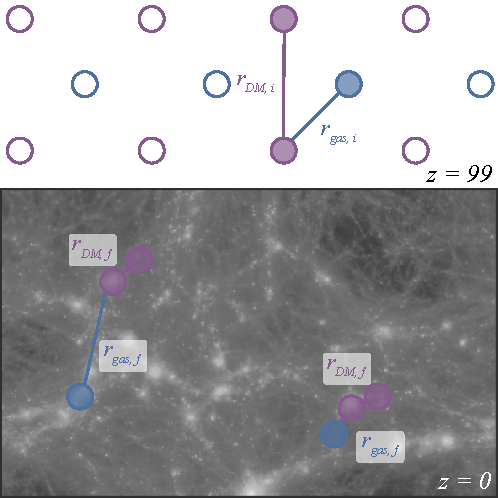
\includegraphics[width=\columnwidth]{figures/kspafig_small.pdf}
    \vspace{-0.5cm}
    \caption{The matching procedure between initial and final conditions
    illustrated. The top panel shows the $z=99$ initial conditions, where
    every particle finds its nearest dark matter neighbour. The bottom
    panel shows the distances between those particles at $z=0$.}
    \vspace{-0.5cm}
    \label{fig:kspafigsmall}
\end{figure}

\begin{figure*}
    \centering
    \includegraphics[width=\textwidth]{figures/distance_figure.pdf}
    \caption{The large-scale structure of the 50 Mpc reference model is shown.
    The background gray colour-map shows the projected column density of the
    gas in the simulation. Over-plotted is 1/250th of all gas particles
    in the simulation, coloured and sized by their distance travelled
    according to the metric below. Note how the low-distance particles
    are those that are trapped in the potential wells of the galaxies
    and clusters present in the simulations, with the particles that
    have travelled farther compared to their dark matter counterpart
    residing, in general, outside of any bound system.}
    \label{fig:feedbackpic}
\end{figure*}

\begin{figure*}
    \centering
    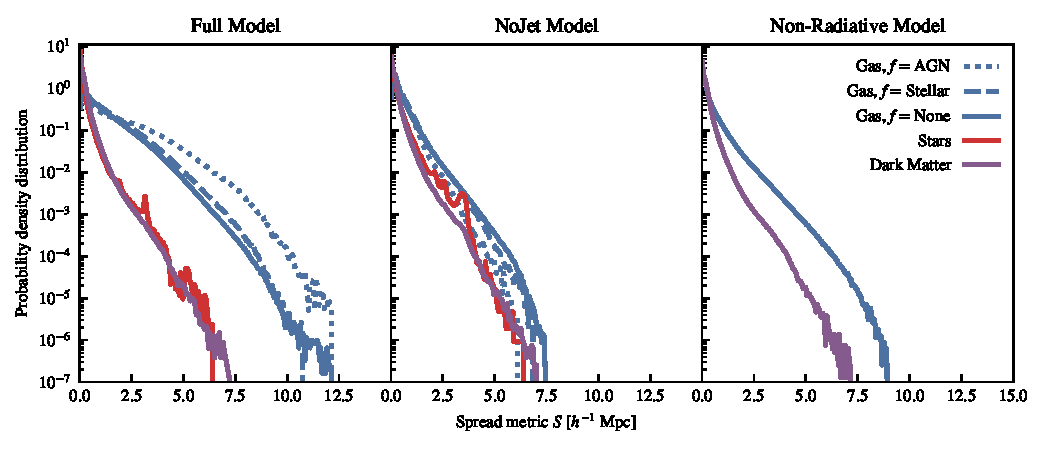
\includegraphics[width=\textwidth]{figures/neighbour_analysis_feedback_histogram_combined.pdf}
    \vspace{-0.7cm}
    \caption{
        The (normalised) distribution of distances for all particles $i$ to
        the nearest neighbour $j$ in the initial conditions, split by particle
        type. This is shown for the $z=0$ particle distribution in the
        reference model (left), \nojet{} model (center), and a non-radiative
        run (right). Splitting the particles by those that have been
        involved in feedback events in this figure shows that the further
        out a particle has been blown the more likely it is to have been
        directly involved in a feedback event for the reference model. Also note
        the vertical $0.5-1$ dex offset for gas compared to dark matter even in
        the \nojet{} run. 
    }\label{fig:feedbackdistance}
\end{figure*}


To investigate the systematic effects of feedback and dynamics on the baryonic
matter in a cosmological simulation, we have developed the following (simple)
spread metric (illustrated in Figure \ref{fig:kspafigsmall}, and visualised in Figure \ref{fig:feedbackpic}):

\begin{enumerate}
	\item For every particle $i$ in the initial conditions, find the nearest
              dark matter neighbour $j$.
	\item In the final conditions, match all remaining baryonic particles
	      with their initial conditions progenitor (in this case, stars are
	      matched with their gas progenitor).
	\item In the final conditions, find the distance $r_{ij}$, i.e. the
	      distance between the original neighbours.
\end{enumerate}

This method is completly independent of rest frame and can also be repeated
for the non-baryonic matter to see the effects of gravitational dynamics. In
experimenting with this metric, it appears that simply taking the base
distance for the nearest neighbour gives nearly equivalent results to taking
the median or mean distance over a number of closest neighbours, and so here
the more simple single distance measure is quoted.

In Figure \ref{fig:feedbackdistance} (left panel) the distribution of
distances in the reference model is shown. Note how similar the stellar
distribution is to the dark matter distribution even though strong feedback is
included; this shows that the star particles are mainly affected by
gravitational dynamics and  are mainly formed from gas that is in the core of
the halo and can only end up distances of around $6 \hmpc{}$. This is
expected, as it is about three times the virial radius of the largest halo in
the simulation; a pair of initially neighbouring particles can end up on
opposite sides of a given halo. The gas, on the other hand, can be blown out
to very large distances (over $12 \hmpc{}$).

Comparing to the \nojet{} run in Figure \ref{fig:feedbackdistance}, it is clear
that the jets have a significant impact on the distances to which particles
are spread. These two plots show directly the issue of entrainment that was
raised earlier; the tail is expanded to include lots of gas that was never
tagged as having been included in any feedback event.

The significant difference in the dynamics between the \nojet{} run and the
reference model is surprsing. Less than $0.4\%$ of gas particles in the simulation
have ever interacted directly with the AGN jets; this has been enough
to completely separate the majority of the gas from the dark matter dynamically.
Such a high degree of separation points to huge amounts of gas being entrained
by these powerful jets; it is not simply the case that higher mass ($M_H >
10^{11} \msolar{}$) halos are quenched internally reducing their star formation
rate; the energetics and dynamics of the CGM and IGM are significantly altered
leading to a much more complex interaction between the turn-off of the
galaxy stellar mass function (GSMF) and the power of the AGN jets.

The final contrast to highlight is the difference between the \nojet{} and
non-radiative model. The non-radiative model shows increased distance between
gas particles and their associated dark matter neighbour compared to the
\nojet{} run; this is likely due to the lack of cooling preventing particles
that lie in small halos from remaining as tightly bound.

These results show that gaseous and stellar matter can be transferred out
to significantly further (by $z=0$) than is assumed by typical zoom-in simulation
suites. For example, the Latte \citep{Wetzel2016} suite uses an exclusion region
for high resolution particles of around $1.5 \hmpc{}$. Whilst they do not find
contamination (possibly due to refinement criteria) of low-resolution particles
into the high-resolution region, the above metrics suggest that perhaps this is
a more numerical, rather than physical, effect; low resolution particles are
not present due to a lack of sub-grid physics in the unrefined region.
